%Ultimatives Tool zur Datierung:
%https://www.cc.kyoto-su.ac.jp/~yanom/pancanga/
%skp = ignored in edition
%skm = ignored in xml
\documentclass[10pt]{memoir}
\setstocksize{220mm}{155mm} 	        
\settrimmedsize{220mm}{155mm}{*}	
\settypeblocksize{170mm}{116mm}{*}	
\setlrmargins{18mm}{*}{*}
\setulmargins{*}{*}{1.2}
%\setlength{\headheight}{5pt}%
\checkandfixthelayout[lines]
\linespread{1.16}
\flushbottom

%%% Hyphenation settings
\usepackage[htt]{hyphenat}
\hyphenation{he-lio-trope opos-sum}
\tracingparagraphs=1
%Hyphenation in Devanāgarī of the edition still missing? Probably this needs to be modified in babel-iast package? 

%%% babel
\usepackage[english]{babel}
\usepackage{babel-iast/babel-iast}

\babelfont[iast]{rm}[Renderer=Harfbuzz, Scale=1.3]{AdishilaSan}%AdishilaSan}
\babelfont[english]{rm}{Adobe Text Pro}

%%% more functionality
\PassOptionsToPackage{hyphens}{url}
\usepackage{hyperref}
\usepackage{pdflscape}
\usepackage{cleveref}
\usepackage{url}
\usepackage{cleveref}
\usepackage{microtype}
\usepackage{lineno}

%\usepackage{bigfoot}
%%% more functions
\usepackage[dvipsnames]{xcolor}
%\usepackage[para,perpage]{footmisc}

%%%für den Counter von Kapiteln und Sätzen! 
\newcommand{\uproman}[1]{\uppercase\expandafter{\romannumeral#1}}
\newcommand{\lowroman}[1]{\romannumeral#1\relax}

\makeindex
\newfontfamily\sanskritfont[Script=Devanagari,Mapping=RomDev,Scale=1.1]{Sanskrit2003}
\usepackage{pifont,fourier-orns,lettrine,psvectorian,paralist,enumitem,pdfpages,wrapfig,tabulary,lettrine,longtable}
\setlist[enumerate]{itemsep=0mm}
\usepackage[autostyle]{csquotes}
\usepackage[defaultlines=2,all]{nowidow}
\usepackage{ellipsis,adforn,booktabs,longtable,url,tikz}
\lineskiplimit=-3pt          

\makechapterstyle{IeT}{%
  \chapterstyle{default}
  \renewcommand*{\printchapternonum}{\centering}
  \renewcommand*{\clearforchapter}{\cleartorecto} 
  \aliaspagestyle{chapter}{empty}}
\chapterstyle{IeT}
\setsecnumdepth{none}  \openright  \nouppercaseheads
\settocdepth{subsubsection}

%%%% test better pagebreaks
%\def\fussy{%
%  \emergencystretch\z@
%  \tolerance 200%
%  \hfuzz .1\p@
%  \vfuzz\hfuzz}

%\interfootnotelinepenalty=10000\relax

%\usepackage[maxfloats=256]{morefloats}

%\maxdeadcycles=500

%raggedbottomsectiontrue
%%\checkandfixthelayout


%%%%%%%  biblatex
%\newcommand{\noun}[1]{\textsc{#1}}    %  philosophy-verbose
\usepackage[backend=biber, sorting=nyt, style=verbose]{biblatex} %%%%ORIGINAL TiE
\renewcommand*{\mkbibnamefamily}[1]{\textsc{#1}}


\DeclareFieldFormat{url}{%
  \mkbibacro{URL}\addcolon\space
  \href{#1}{\nolinkurl{\thefield{urlraw}}}}

\DeclareFieldFormat{citeurl}{%
  \href{#1}{\nolinkurl{\thefield{urlraw}}}} 


\DeclareFieldFormat{postnote}{#1}
\renewcommand{\postnotedelim}{, }
\addbibresource{bindu.bib}

%%% ekdosis
\usepackage[teiexport=tidy,parnotes=true]{ekdosis}% =tidy cleans up HTML and XML documents by fixing markup errors and upgrading legacy code to modern standards. parnotes=footnotes below or above critical apparatus

\SetLineation{lineation=page, modulo} %lineation=page sets thenumbering to start afresh at the top of each page. =modulo makes every fifth line numbered. {lineation=page} makes every line numbered! 

\renewcommand{\linenumberfont}{\selectlanguage{english}\footnotesize} %sets language of lines to English

\SetTEIxmlExport{autopar=false} %autopar=falseinstructs ekdosis to ignore blank lines in the.tex sourcefile as markers for paragraph boundaries. As a result, each paragraph of the edition must be found within an environment associated with the xml <p> element

\SetHooks{
  lemmastyle=\bfseries,
  %refnumstyle=\selectlanguage{english}\bfseries,
  refnumstyle=\selectlanguage{english}\color{blue}\bfseries,
  appheight=0.8\textheight,
}

\newif\ifinapparatus
\DeclareApparatus{source}[
%bhook=\inapparatustrue,
lang=english,
notelang=english,
% bhook=\selectlanguage{english},
bhook=\selectlanguage{english}\textbf{Sources:},%
%maxentries=4, 
%ehook=.]
%sep={] },
%nosep,
]

\newif\ifinapparatus
\DeclareApparatus{testium}[
%bhook=\inapparatustrue,
lang=english,
notelang=english,
% bhook=\selectlanguage{english},
bhook=\selectlanguage{english}\textbf{Testimonia:},
%maxentries=4, 
%ehook=.]
%nosep, 
]

% Declare \ifinapparatus and set \inapparatustrue at the beginning of
% the apparatus criticus block. Also set the language.  
\newif\ifinapparatus
  \DeclareApparatus{default}[
  %bhook=\inapparatustrue, 
  lang=english,
  %maxentries=33,
  %bhook=\selectlanguage{english},
  sep = {] },
  delim=\hskip 0.75em,
  rule=\rule{0.7in}{0.4pt},
]

\newif\ifinapparatus
\DeclareApparatus{philcomm}[
%bhook=\inapparatustrue,
lang=english,
notelang=english,
bhook=\selectlanguage{english}\textbf{Philological Commentary:},
%bhook=\selectlanguage{english},
sep={: },
]

\ekdsetup{
showpagebreaks,
spbmk = \textcolor{blue}{spb},
hpbmk = \textcolor{red}{hpb}
}

%\usepackage{fnpos}
%\makeFNmid
%\makeFNbottom
\usepackage[bottom]{footmisc}
%%%%%%%%%%%%%%%%%%%%%%%%%%%
\makeatletter
\def\blfootnote{\gdef\@thefnmark{}\@footnotetext}
\makeatother
%%%%%%%%%%%%%%%%%%%%%%%%%


% Macros and Definitions for the Print of Sigla
\def\acpc#1#2#3{{#1}\rlap{\textrm{\textsuperscript{#3}}}\textsubscript{\textrm{#2}}\space}
\def\sigl#1#2{{{#1}}\textsubscript{\textrm{#2}}}
\def\None{{\sigl{N}{1}}} \def\Noneac{\acpc{N}{1}{ac}\,} \def\Nonepc{\acpc{N}{1}{pc}\,}
\def\Ntwo{{\sigl{N}{2}}} \def\Noneac{\acpc{N}{2}{ac}\,} \def\Nonepc{\acpc{N}{2}{pc}\,}
\def\Done{{\sigl{D}{1}}} \def\Doneac{\acpc{D}{1}{ac}\,} \def\Donepc{\acpc{D}{1}{pc}\,}
\def\Dtwo{{\sigl{D}{2}}} \def\Dtwoac{\acpc{D}{2}{ac}\,} \def\Dtwopc{\acpc{D}{2}{pc}\,}
\def\Uone{{\sigl{U}{1}}} \def\Uoneac{\acpc{U}{1}{ac}\,} \def\Uonepc{\acpc{U}{1}{pc}\,}                 
\def\Utwo{{\sigl{U}{2}}} \def\Utwoac{\acpc{U}{2}{ac}\,} \def\Utwopc{\acpc{U}{2}{pc}\,}

%%%%%%%%%%%%%% Tattvabinduyoga - List of Witnesses   %%%%%%%%%%%%%%%%%%%
\DeclareWitness{ceteri}{\selectlanguage{english}cett.}{ceteri}[]   
\DeclareWitness{E}{\selectlanguage{english}E}{Printed Edition}[]    
\DeclareWitness{P}{\selectlanguage{english}P}{Pune BORI 664}[]  
\DeclareWitness{B}{\selectlanguage{english}B}{Bodleian 485}[]       
\DeclareWitness{N1}{\selectlanguage{english}N\textsubscript{1}}{NGMPP 38/31}[]
\DeclareWitness{N2}{\selectlanguage{english}N\textsubscript{2}}{NGMPP B 38/35}[]
\DeclareWitness{L}{\selectlanguage{english}L}{LALCHAND 5876}[]  
\DeclareWitness{D}{\selectlanguage{english}D}{IGNCA 30019}[] 
%\DeclareWitness{D2}{\selectlanguage{english}D\textsubscript{2}}{IGNCA 30020}[]  
\DeclareWitness{U1}{\selectlanguage{english}U\textsubscript{1}}{SORI 1574}[] 
\DeclareWitness{U2}{\selectlanguage{english}U\textsubscript{2}}{SORI 6082}[]
%%%%%%%%%%%%%% Tattvabinduyoga - Groups of Witnesses   %%%%%%%%%%%%%%%%%%%
\DeclareWitness{X}{\selectlanguage{english}\alpha}{Alpha Group: D,N1,N2,U1}[]
\DeclareWitness{Y}{\selectlanguage{english}\beta}{Beta Group: B,E,L,P,U2}[]
%%%%%%%%%%%%% Testimonia
\DeclareWitness{Ysv}{\selectlanguage{english}Ysv}{Yogasvarodaya}[] %%%add infos!  

%%%%%%%%%%%%%%%%%%%%%%%%%%%%%%%%%%%%%%%%%%%
% Macro for Editing Abbrevs.
\def\om{\textrm{\footnotesize \textit{om.}\ }} %prints om. for omitted in apparatus
\def\korr{\textrm{\footnotesize \textit{em.}\ }} %prints em. for emended in apparatus
\def\conj{\textrm{\footnotesize \textit{conj.}\ }} %prints conj. for conjectured in apparatus

% \supplied{text} EDITORIAL ADDITION -> Within \lem oder \rdg
% \surplus{text} EDITORIAL DELETION -> Within \lem oder \rdg
% \sic{text} CRUX
% \gap{text} LACUNAE -> [reason=??, unit=??, quantity=??, extent=??]


%%%%%%%%%%%%%%%%%%%%%%%%%%%%%%%%%%%%%%%%%%% All macros of this list can be used in 
% Macro for Editing Abbrevs.
\def\eyeskip{\textrm{{ab.\,oc. }}}
\def\aberratio{\textrm{{ab.\,oc. }}}
\def\ad{\textrm{{ad}}}
\def\add{\textrm{{add.\ }}}
\def\ann{\textrm{{ann.\ }}}
\def\ante{\textrm{{ante }}} 
\def\post{\textrm{{post }}}
%\def\ceteri{cett.\,}                   
\def\codd{\textrm{{codd.\ }}}

\def\coni{\textrm{{coni.\ }}}
\def\contin{\textrm{{contin.\ }}}
\def\corr{\textrm{{corr.\ }}}
\def\del{\textrm{{del.\ }}}
\def\dub{\textrm{{ dub.\ }}}

\def\expl{\textrm{{explic.\ }}} 
\def\explica t{\textrm{{explic.\ }}}
\def\fol{\textrm{{fol.\ }}}
\def\foll{\textrm{{foll.\ }}}
\def\gloss{\textrm{{glossa ad }}}
\def\ins{\textrm{{ins.\ }}}      
\def\inseruit{\textrm{{ins.\ }}} 
\def\im{{\kern-.7pt\lower-1ex\hbox{\textrm{\tiny{\emph{i.m.}}}\kern0pt}}} %\textrm{\scriptsize{i.m.\ }}}      
\def\inmargine{{\kern-.7pt\lower-.7ex\hbox{\textrm{\tiny{\emph{i.m.}}}\kern0pt}}}%\textrm{\scriptsize{i.m.\ }}}      
\def\intextu{{\kern-.7pt\lower-.95ex\hbox{\textrm{\tiny{\emph{i.t.}}}\kern0pt}}}%\textrm{\scriptsize{i.t.\ }}}           
\def\indist{\textrm{{indis.\ }}}  
\def\indis{\textrm{{indis.\ }}}
\def\iteravit{\textrm{{iter.\ }}} 
\def\iter{\textrm{{iter.\ }}}
\def\lectio{\textrm{{lect.\ }}}   
\def\lec{\textrm{{lect.\ }}}
\def\leginequit{\textrm{{l.n. }}} 
\def\legn{\textrm{{l.n. }}}
\def\illeg{\textrm{{l.n. }}}

\def\primman{\textrm{{pr.m.}}}
\def\prob{\textrm{{prob.}}}
\def\rep{\textrm{{repetitio }}}
\def\secundamanu{\textrm{\scriptsize{s.m.}}}            \def\secm{{\kern-.6pt\lower-.91ex\hbox{\textrm{\tiny{\emph{s.m.}}}\kern0pt}}}%   \textrm{\scriptsize{s.m.}}}
\def\sequentia{\textrm{{seq.\,inv.\ }}}  
\def\seqinv{\textrm{{seq.\,inv.\ }}}
\def\order{\textrm{{seq.\,inv.\ }}}
\def\supralineam{{\kern-.7pt\lower-.91ex\hbox{\textrm{\tiny{\emph{s.l.}}}\kern0pt}}} %\textrm{\scriptsize{s.l.}}}
\def\interlineam{{\kern-.7pt\lower-.91ex\hbox{\textrm{\tiny{\emph{s.l.}}}\kern0pt}}}   %\textrm{\scriptsize{s.l.}}}
\def\vl{\textrm{v.l.}}   \def\varlec{\textrm{v.l.}} \def\varialectio{\textrm{v.l.}}
\def\vide{\textrm{{cf.\ }}}
\def\cf{\textrm{{cf.\ }}} 
\def\videtur{\textrm{{vid.\,ut}}}
\def\crux{\textup{[\ldots]} }
\def\cruxx{\textup{[\ldots]}}
\def\unm{\textit{unm.}}
%%%%%%%%%%%%%%%%%%%%%%%%%%%%%%%%%%%%

% List of Scholars
\DeclareScholar{ego}{ego}[
forename=Nils Jacob,
surname=Liersch]

% Persons:14\DeclareScholar{ego}{ego}[15forename=Robert,16surname=Alessi]17% Useful shorthands:18\DeclareShorthand{codd}{codd.}{V,I,R,H}19\DeclareShorthand{edd}{edd.}{Lit,Erm,Sm}20\DeclareShorthand{egoscr}{\emph{scripsi}}{ego}

%Useful shorthands:
%\DeclareShorthand{codd}{codd.}{V,I,R,H}
%\DeclareShorthand{edd}{edd.}{Lit,Erm,Sm}
\DeclareShorthand{egoscr}{em.}{ego}
\DeclareShorthand{egoscrconj}{conj.}{ego}
\DeclareShorthand{egomute}{\unskip}{ego}

\usepackage{xparse}

\NewDocumentEnvironment{tlg}{O{}O{}}{\setlength{\leftskip}{0pt}\vspace{-1ex}\begin{quotation}}{\hfill #1\ \vspace{-1ex}\end{quotation}\vspace{-1ex}} %verse environment
%\NewDocumentEnvironment{tlg}{O{}O{}}{\begin{verse}}{॥#1\hskip-4pt ॥\\ \end{verse}}
\NewDocumentCommand{\tl}{m}{{\selectlanguage{iast} #1}}

\NewDocumentCommand{\extra}{m}{{\textcolor{gray}{#1}}} %command for additions to U2
\NewDocumentCommand{\crazy}{m}{{\textcolor{red}{#1}}} %totally corrupted passage
\NewDocumentCommand{\coro}{m}{{\textcolor{violet}{#1}}} %colour for sentence counter! 

\NewDocumentEnvironment{prose}{O{}}{\begin{otherlanguage}{iast}}{\end{otherlanguage}}
% \NewDocumentEnvironment{padd}{O{}}{\begin{otherlanguage}{iast}}{\end{otherlanguage}}
\NewDocumentEnvironment{tlate}{O{}}
%\NewDocumentEnvironment{tadd}{O{}}

%Define two commands: \skp ("sanskrit plus"), to be ignored by TeX in
%the edition text, but processed in the TEI output. Conversely, \skm
%("sanskrit minus") is to be processed in the edition text, but
%ignored if found in the apparatus criticus and in the TEI output:

\NewDocumentCommand{\skp}{m}{}
\TeXtoTEIPat{\skp {#1}}{#1}

%\NewDocumentCommand{\skpp}{m}{}
%\TeXtoTEIPat{\skpp {#1}}{#1}

\NewDocumentCommand{\skm}{m}{\unless\ifinapparatus#1-\fi}
\TeXtoTEIPat{\skm {#1}}{}

% \NewDocumentCommand{\dd}{}{/\hskip-4pt/}
\NewDocumentCommand{\dd}{}{\mbox{/\hskip-4pt/}}
\TeXtoTEIPat{\dd {}}{//}


%%% modify environments and commands
%%% TEI mapping
\TeXtoTEIPat{\begin {tlg}}{<lg>} %lg=(Group of verse (s)) contains one or more verses or lines of verse that together form a formal unit (e.g. stanza, chorus).
\TeXtoTEIPat{\end {tlg}}{</lg>}

\TeXtoTEIPat{\begin {prose}}{<p>}
\TeXtoTEIPat{\end {prose}}{</p>}

\TeXtoTEIPat{\begin {tlate}}{<p>}
\TeXtoTEIPat{\end {tlate}}{</p>}

\TeXtoTEIPat{\\}{}
\TeXtoTEIPat{\linebreak}{<br/>}
\TeXtoTEIPat{\noindent}{}
%\TeXtoTEI{tl}{l}
\TeXtoTEI{emph}{hi}
\TeXtoTEI{bigskip}{}
\TeXtoTEI{None}{N1}
\TeXtoTEI{Ntwo}{N2}
\TeXtoTEI{Done}{D1}
\TeXtoTEI{Dtwo}{D2}
\TeXtoTEI{Uone}{U1}
\TeXtoTEI{Utwo}{U2}
%\TeXtoTEIPat{/}{ |}
%\TeXtoTEI{//}{ ||}
\TeXtoTEIPat{\korr}{em. }
\TeXtoTEIPat{\conj}{conj.}
\TeXtoTEIPat{\om}{om.}
\TeXtoTEIPat{english}{}
\TeXtoTEIPat{\hskip}{}
\TeXtoTEIPat{\hskip-4pt}{}
\TeXtoTEIPat{\hskip-2pt}{}
\TeXtoTEIPat{-}{ }
\TeXtoTEIPat{4pt}{}
\TeXtoTEIPat{2pt}{}
\TeXtoTEIPat{\textcolor {#1}{#2}}{<hi rend="#1">#2</hi>} 

% Nullify \selectlanguage in TEI as it has been used in
% \DeclareWitness but should be ignored in TEI.
\TeXtoTEI{selectlanguage}{}



\FormatDiv{1}{\begin{center}\Large}{\end{center}}
\FormatDiv{2}{\begin{center}\small}{\end{center}}
\FormatDiv{3}{\bfseries}{.}
\title{Tattvayogabindu of Rāmacandra\\ A Critical Edition and Annotated Translation\\ and a Comparative Analysis of the \\Complex Early Modern Yoga Yaxonomies }
\date{\today}
\parindent=15pt

\begin{document}

\frontmatter
\thispagestyle{empty} % Verhindert Seitenzahl auf der Seite
\begin{center}

%\vspace{0.5in}

%\begin{otherlanguage}{iast}
%   \large\sanskritfont{Tattvayogabindu}\\
%\end{otherlanguage}

\vspace{0.25in}


\huge\textbf{\MakeUppercase{The Tattvayogabindu \\of Rāmacandra}}\\

\vspace{0.2in}

\Large  Critical Edition and Annotated Translation of an Early Modern Text on Rājayoga, with a Comparative Analysis of the Complex Yoga Taxonomies from the Same Period\\ 

\vspace{0.45in}

\thispagestyle{empty}
\end{center}
%\newpage
%\thispagestyle{empty}
%\mbox{}
%\newpage

\newpage

  \thispagestyle{empty}
  \begin{figure}[p]
    \centering
    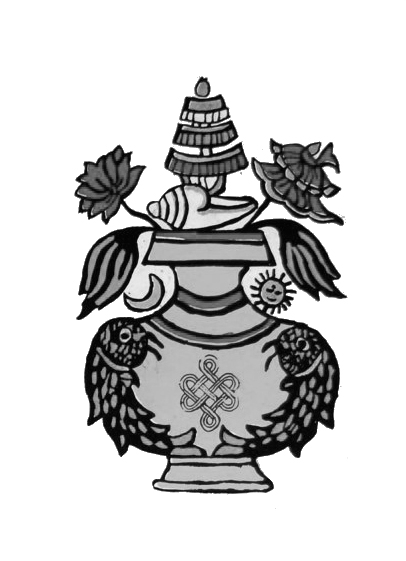
\includegraphics[width=0.25\textwidth]{pics/purna.jpg}
  \end{figure}
  
\newpage

\begin{landscape}
\thispagestyle{empty}
  \begin{figure}[p]
	\centering
  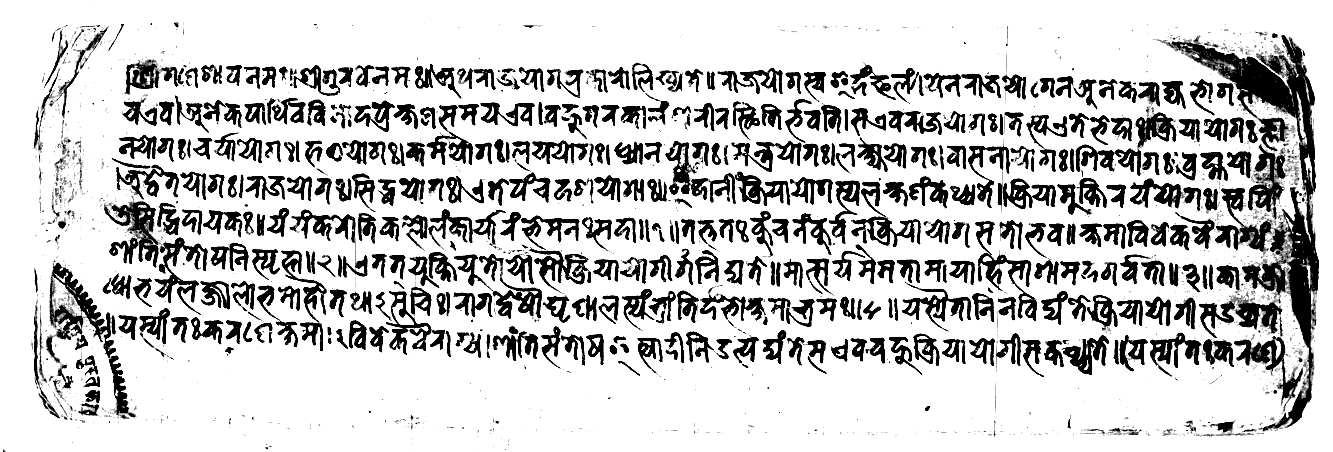
\includegraphics[width=1.5\textwidth]{pics/folio1.jpg}
	\caption{Folio 1v of Ms. \getsiglum{N1}.}
	 \phantomsection\label{fig_folio1}
\end{figure}
\end{landscape}

\cleardoublepage
\tableofcontents
\thispagestyle{empty}
\newpage 
\listoffigures
\thispagestyle{empty}
\newpage
\listoftables
\thispagestyle{empty}
\newpage

\mainmatter
\pagestyle{defaultstyle}
\counterwithout{footnote}{chapter}
\counterwithout{figure}{chapter}
\counterwithout{table}{chapter}
\renewcommand{\thetable}{\arabic{table}}
%%%tables 
\setsecnumdepth{section}
\maxsecnumdepth{subsubsection}
\newpage
\chapter{Introduction}
\cleardoublepage

\section{General remarks}
 \phantomsection\label{generalremarks}
 \lettrine{T}{he} \textit{Tattvayogabindu} of Rāmacandra\footnote{A discussion about the author Rāmacandra is found on p. \pageref{ramarama}.} is an early modern Sanskrit text on Rājayoga that was written in the first half of the seventeenth century\footnote{The dating of the text is discussed on p. \pageref{dating}.} in northern India.\footnote{The detailed discussion of the place of origin is found on p. \pageref{riversrivers}, n. \ref{riversrivers}.} The most salient feature of the work that makes it historically significant is its highly differentiated taxonomy of types of yoga.\footnote{This is a remarkable increase in the number of declared yogas compared to the standard medieval tetrad of Mantra, Laya, Haṭha and Rājayoga.} In the \textit{Tattvayogabindu}'s introduction, most manuscripts name fifteen types of yoga, presented as methods of Rājayoga. These are 1. Kriyāyoga, 2. Jñānayoga, 3. Caryāyoga, 4. Haṭhayoga, 5. Karmayoga, 6. Layayoga, 7. Dhyānayoga, 8. Mantrayoga, 9. Lakṣyayoga, 10. Vāsanāyoga, 11. Śivayoga, 12. Brahmayoga, 13. Advaitayoga, 14. Siddhayoga, and 15. Rājayoga itself. The text is a yogic compendium written in a mix of mainly prose and 47 verses in textbook-style, where its 59 topics are introduced in sections most of the time launched by recognizable phrases. The sections deal with the methods of Rājayoga and their effects, but others also cover topics like yogic physiology, the Avadhūta, the importance of the guru, cosmogony, and a \textit{yogaśāstrarahasya}.  

The \textit{Tattvayogabindu} has not been discussed comprehensively or considered in the secondary literature on yoga. The only exception is \citeauthor{birch2014} (2014: 415–416) who briefly described its list of fifteen yogas in the context of the ``fifteen medieval yogas'' and noted that a similar taxonomy occurs in Nārāyaṇatīrtha’s \textit{Yogasiddhāntacandrikā} (17th century), a commentary on the \textit{Pātañjalayogaśāstra} that integrates fifteen medieval yogas within its \textit{aṣṭāṅga} format. An incomplete account of the fifteen yogas is found within the Sanskrit yoga text \textit{Yogasvarodaya}, which is known only through quotations in the \textit{Prāṇatoṣinī}, the \textit{Yogakarṇikā} and the \emph{Śabdakalpadruma}.\footnote{Manuscripts under the name of \textit{Yogasvarodaya} seem to be lost. I was not able to locate the manuscripts of the text in any manuscript catalogue at hand.} The \textit{Yogasvarodaya} announces a total of fifteen yogas but names only eight of them in its introductory \textit{śloka}s. It is the primary source and template for the compilation of the \textit{Tattvayogabindu}. Besides several passages, Rāmacandra, in many instances, follows its content and structure by rewriting the \textit{Yogasvarodaya}’s \textit{śloka}s into prose or quoting them directly without attribution. Due to the incomplete transmission of the \textit{Yogasvarodaya}, Rāmacandra’s \textit{Tattvayogabindu} is a natural and valuable starting point for an unprecedented in-depth study of the complex early modern yoga taxonomies, a phenomenon that can be narrowed down precisely in terms of time and as I will show regarding its localisation. The other source text that Rāmacandra used is the \textit{Siddhasiddhāntapaddhati} whose content he draws on, particularly in the second half of his composition. Another text that includes an almost similar taxonomy of twelve yogas divided into three tetrads\footnote{See p.\pageref{sarvasarva} for a detailed discussion of the \textit{Sarvāṅgayogapradīpikā}.} is Sundardās’s \textit{Brajbhāṣā} yoga text named \textit{Sarvāṅgayogapradīpikā} which not just shares most of the types of yogas but also provides a different and valuable perspective on the addressed yoga categories.\footnote{For a comparative table of the complex early modern yoga taxonomies see table \ref{tab:complextaxonomies} on p. \pageref{tab:complextaxonomies}.}

These complex taxonomies that emerged during the 17th century crossed sectarian divides and were adapted to the specific needs of different authors and traditions. The \textit{Tattvayogabindu} thus encapsulates a large proportion of the diversity of yoga types and teachings after the \textit{Haṭhapradīpikā} (15th century) that were adopted and practised by a broad spectrum of religious traditions and strata of Indian society. In the particular case of the \textit{Tattvayogabindu}, there are various statements throughout the text that reveal a strategy to detach yoga from its ascetic and renunciate connotations and to stylise Rājayoga as a practice that can bring the desired soteriological benefits even to practitioners who enjoy worldly pleasures and expensive lifestyles. Textual evidence suggests that the \textit{Tattvayogabindu} is an important example of a text that provides an early modern adaptation of Rājayoga for \textit{kṣatriya}s in a courtly environment.

One printed edition of the \textit{Tattvayogabindu} was published in 1905 with a Hindi translation and based on (an) unknown manuscript(s).\footnote{\emph{Binduyoga}. \textit{Binduyogaḥ with Bhāṣaṭīkā}. Ed. by Jvālāprasāda Miśra. Mumbai, 1905.} This publication has the title ``\textit{Binduyoga}'' confirmed by the printed text’s colophon. However, as I will discuss in the introduction, the text was originally known as \textit{Tattvayogabindu}. The consulted manuscripts contain significant discrepancies, structural differences and variant readings between them and the printed edition.\footnote{For example, the printed edition does not contain the complex yoga taxonomy presented in the manuscripts of the \emph{Tattvayogabindu}.} Furthermore, the manuscripts are scattered over the northern half of the Indian subcontinent and Nepal, which suggests that the text was widely transmitted at some point. Lengthy passages of the \textit{Tattvayogabindu} are quoted without attribution in a text called \textit{Yogasaṃgraha} and Sundaradeva’s \textit{Haṭhasaṅketacandrikā}.

The first chapter of this dissertation contains a general introduction to Rāmacandra's \textit{Tattvayogabindu}. The chapter gives a brief overview of the content of the text and discusses its origin, the author and the author's intended audience. Subsequently, the textual witnesses, source texts and testimonies of the \textit{Tattvayogabindu} are described. A stemmatic analysis of the text is then presented, based on manual philological observation and computer-assisted stemmatics to present a \textit{stemma codicum}. The chapter concludes with a presentation of the editorial policies, which form the basis for the second chapter of this thesis.
The second chapter, the core of this dissertation, is a critical edition and annotated translation of the \textit{Tattvayogabindu}. The critical edition significantly improves the text and sheds new light on its historical significance.
The third chapter contains a comparative analysis of the complex early modern yoga taxonomies based on hermeneutics of difference.\footnote{The conceptof hermeneutics of difference is discussed on p. \pageref{hermeneutics}, n. \ref{hemerneutics}.}  Using the new critical edition of the \textit{Tattvayogabindu} and the texts mentioned above, \emph{Yogasvarodaya}, \emph{Yogasiddhāntacandrikā} and \emph{Sarvāṅgayogapradīpikā}, the complex yogic taxonomies of the four texts are compared in detail. Based on this comparative analysis, a differentiated hypothesis on the emergence of the complex yoga taxonomies was developed, and the complex yoga taxonomies were located und explained in the broader context of the historical development of the yoga traditions. The comparison includes a nuanced description of each yoga category used by the authors of the texts with complex yoga taxonomies. While the authors of the four texts often operate with identical terms for the individual yoga categories, they interpret these categories according to their religious backgrounds and agendas, with intriguing and exciting differences. Contrasting the comparanda, i.e. the authors, the texts, the yoga taxonomies and the yoga categories, therefore provides a deep insight into the discursive negotiation processes of the Indian yoga traditions of the 17th century.


\chapter{Conventions in the Critical Apparatus}
\section{Sigla in the Critical Apparatus}

\begin{itemize}
\item \beta : \getsiglum{D}, \getsiglum{J}, \getsiglum{K1}, \getsiglum{N1}, \getsiglum{N2}, \getsiglum{U1}
\item \gamma : \getsiglum{B}, \getsiglum{E}, \getsiglum{L}, \getsiglum{P}, \getsiglum{U2}
\item B : Bodleian Oxford D 4587
\item C : \emph{Haṭhasaṅketacandrikā} GOML Ms. No. R 3239
\item C\textsubscript{pc} : \emph{Haṭhasaṅketacandrikā} GOML Ms. No. R 3239
\item cett.: ceteri (all manuscripts except the ones mentioned in the lemma)
\item \Done : IGNCA 30019
\item E : Printed Edition
\item J : JNUL Ms. No. 55769
\item Jo : \emph{Haṭhasaṅketacandrikā} MMPP MS. No. 2244
\item \Kone : AS G 11019
\item L : Lalchand Research Library LRL5876
\item M : \emph{Haṭhasaṅketacandrikā} ORI Ms. No. B 220
\item \Ntwo : NGMPP B 38-35 / A 1327-14
\item \None : NGMPP B 38-31
\item P : Pune BORI 664
\item PT : \emph{Prāṇatoṣiṇī}
\item \Uone : SORI 1574
\item \Utwo : SORI 6082
\item V : OI MSU 10558
\item YK : \emph{Yogakarṇikā}% 
\item YSv : \emph{Yogasvarodaya}
\end{itemize}
\newpage

\chapter[Critical Edition \& Annotated Translation of the \emph{Tattvayogabindu}]{The \emph{Tattvayogabindu} of Rāmacandra \\ \huge  
  Critical Edition \& Annotated Translation}
\pagestyle{chapter2style}
\newpage
\begin{alignment}[
  texts=edition[class="edition"];
  translation[class="translation"],
  ]
  \begin{edition}
    \ekddiv{
      head={[\uproman{30}. \textbf{ādhāracakrasya bhedāḥ}]},
      type=section,
      depth=2, 
      n=XXX
    }
    \xmlhead[h30]{[XXX. ādhāracakrasya bhedāḥ]}
    \phantomsection
    \addcontentsline{toc}{section}{XXX. ādhāracakrasya bhedāḥ}
 \begin{prose}[p30_01]
   \noindent
%-----------------------------
%idānīm ādhāracakrasya bhedāḥ kathyanta/   \E
%idānīm ādhāracakrasya bhedaḥ kathyate     \P
%idānīm ādhāracakrasya bhedā  kathyaṃte/    \B DSCN7165.jpg Z.3
%idānīm ādhāracakrasya bhedā  kathyaṃte//   \L
%idānīm ādhāracakrasya bhedaḥ kathyate/    \N1
%idānīṃ ādhāracakrasya bhedaḥ kathyate//   \D
%idānīṃ ādhāracakrasya bhedaḥ kathyate//   \K1
%idānīṃ ādhāracakrasya bhedāḥ kathyate//   \J   
%idānī  ādhāracakrasya bhedaḥ kathyaṃte/   \N2
%idānīṃ ādhāracakrasya bhedāḥ kathyaṃte    \U1
%idānīṃ ādhāracakrasya bhedāḥ kathyaṃte // \U2
%-----------------------------
%Now the divisions of the totality of container [for concentration] are taught.
%-----------------------------
   \note[type=source, labelb=_75b, labele=_75e, nosep]{cf. YSv (PT, p. 839) = YK 2.15: ṣoḍaśādhārabhedan tu śṛṇu devi viśeṣataḥ |}
   \note[type=source, labelb=_75b, labele=_75e, nosep]{cf. SSP 2.10 (Ed. p. 32): atha ṣoḍaśādhārāḥ kathyante |}
   \note[type=testium, labelb=_75b, labele=_75e, nosep]{cf. \citetitle{hathasamketacandrikajodhpur} (MMPP 2244 f. 98r ll. 3-4): ity ādhārāḥ ṣodaśayaṃ athoktānāṃ ṣoḍaśādhārāṇāṃ kartavyatām āha |}
\app{\lem[wit={ceteri}, alt={idānīm}]{idānī\skp{m-ā}}\linelabel{_75b}
  \rdg[wit={N2}]{idānī}
}\skm{m-ā}dhāracakrasya
\app{\lem[wit={ceteri}]{bhedāḥ}
  \rdg[wit={B,L}]{bhedā}}
\app{\lem[wit={ceteri}]{kathyante}
  \rdg[wit={E}]{kathyanta}
  \rdg[wit={D,N1}]{kathyate}}/\linelabel{_75e}
%-----------------------------
%pādayor aṃguṣṭhe  tejaso  lakṣyakāraṇāt              dṛṣṭiḥ sthirā bhavati/ \E
%pādayor aṃguṣṭhe  tejaso  lakṣyakaraṇāt              dṛṣṭiḥ sthirā bhavati  \P
%pādayor aṃguṣṭhai tejasaṃ lakṣaṃ kartavyaṃ kāraṇāt// dṛṣṭiḥ sthirā bhavati/ \B
%pādayor aṃguṣṭhe  tejasaṃ lakṣaṃ karttavyaṃ kāraṇāt  dṛṣṭiḥ sthirā bhavatī/ \L
%pādayor aṃguṣṭhe  tejaso  lakṣyakāraṇāt              dṛṣṭisthirā   bhavati/ \N1
%pādayor aṃguṣṭhe  tejaso  lakṣyakāraṇāt              dṛṣṭiḥ sthirā bhavati \D
%pādayor aṃguṣṭhe  tejaso  lakṣyakāraṇāt//            dṛṣṭiḥ sthirā bhavati \K1
%pādayor aṃguṣṭhe  tejaso  lakṣyakāraṇāt              dṛṣṭiḥ sthirā bhavati// \J
%pādayor aṃguṣṭhe  tejaso  lakṣakāraṇāt               dṛṣṭisthirā   bhavati/ \N2
%pādayor aṃguṣṭhe  tejaso  lakṣyakāraṇāt              dṛṣṭisthirā   bhavati \U1
%pādayor aṃguṣṭhe  tejaso  lakṣyakāraṇāt              dṛṣṭisthirā   bhavati// \U2 %%%415.jpg
%-----------------------------
%From the execution of the fixation onto the light at the big toe of the feet stability of the gaze arises.
%-----------------------------
\note[type=source, labelb=_76b, labele=_76e, nosep]{cf. YSv (PT, p. 839): aṅguṣṭhapādayos tejaḥ salakṣasthiradṛṣṭimān | pādāṅguṣṭhe ya ādhāraḥ prathamo (\textit{prathamaṃ} YK 2.16) yogatattvataḥ |}
\note[type=source, labelb=_76b, labele=_76e, nosep]{cf. SSP 2.10 (Ed. p. 32): tatra prathamaḥ pādāṅguṣṭhādhāraḥ | tatrāgratas tejomayaṃ dhyāyet | dṛṣṭiḥ sthirā bhavati |}
\note[type=testium, labelb=_76b, labele=_76e, nosep]{ \approx  \citetitle{hathasamketacandrikajodhpur} (MMPP 2244 f. 98r l. 4): tatra mūlādhāraḥ 1 pādayor aṃguṣṭhe tejaso lakṣyakaraṇād dṛṣṭiḥ sthirā bhavati 2 ity ādhāracakraṃ |}
pādayo\skp{r-aṃ}\app{\lem[wit={ceteri}, alt={aṅguṣṭhe}]{\skm{r-aṅ}guṣṭhe}\linelabel{_76b}
  \rdg[wit={B}]{aṃguṣṭhai}}
\app{\lem[wit={ceteri}]{tejaso}
  \rdg[wit={B,L}]{tejasaṃ}}
\app{\lem[wit={ceteri}, alt={lakṣya°}]{lakṣya}
  \rdg[wit={N2}]{lakṣa°}
  \rdg[wit={B,L}]{lakṣaṃ kartavyaṃ}
}\app{\lem[wit={ceteri}, alt={°kāraṇād}]{kāraṇā\skp{d-dṛ}}
    \rdg[wit={P}]{°karaṇāt}
  }\app{\lem[wit={ceteri}, alt={dṛṣṭiḥ}]{\skm{d-dṛ}ṣṭiḥ}
   \rdg[wit={N1,N2,U1,U2}]{dṛṣṭi°}} sthirā
 \app{\lem[wit={ceteri}]{bhavati}
   \rdg[wit={L}]{bhavatī}}/\linelabel{_76e}
%-----------------------------
%dvitīyo mūlādhāraḥ/  pādāṃguṣṭhasya mūle parapādasya  pārṣṇiḥ                                         sthāpyate tadāgniḥ prabalo bhavati/ \E
%dvitīyo mūlādhāraḥ   pādāṃguṣṭhasya mūle 'parapādasya dhāraḥ pādāṃduṣṭhasya mūleḥ parapādasya pārṣṇiḥ sthāpyate tadāgniḥ prabalo bhavati \P
%dvitīyo mūlādhāraḥ/  pādāṃguṣṭhasya mūle aparasya pādapārṣṇiḥ                                         syāpyate tadāgniḥ  prabalo bhavatī/ \B
%dvitīyo mūlādhāraḥ   pādāṃguṣṭhasya mūle aparasya pādapārṣṇīḥ                                         syāpyate tadāgniḥ  prabalo bhavatī/ \L
%dvitīyo mūlādhāraḥ/  pādāṃguṣṭhasya mūle aparapādasya pārṣṇiḥ                                         sthāpyate agniḥ    prabalo bhavati/   \N1
%dvitīyo mūlādhāraḥ// pādāṃguṣṭhasya mūle aparapādasya pārṣṇiḥ                                         sthāpyate agni-----prabalo bhavati//   \D  %%%p.12 recto
%dvitīyo mūlādhāraḥ// pādāṃguṣṭhasya mūle aparapādasya pārṣṇi                                         sthāpyate agni-----prabalo bhavati//   \K1
%dvitīyo mūlādhāraḥ pādāṃguṣṭhasya mūle adharapādasya pārṣṇiḥ                                         sthāpyate// agniprabalo bhavati//   \J 
%dvitīyo mūlādhāraḥ   pādāṃguṣṭhasya mūle aparapādasya pārṣṇiḥ                                         sthāpyate/ \om                     \N2
%dvitīyo mūlādharaḥ   pādāṃguṣṭhasya mūle aparapādasya pārṣṇiḥ                                         sthāpyate agniṃ ---prabalo bhavati    \U1
%dvitīyo mūlādhare    pādāṃguṣṭhasya mūle 'parapādasya pārṣṇiḥ                                         sthāyyaṃte//                       \U2
%-----------------------------
%The second root-container is the second [one]. The heel of the other foot is caused to be placed at the root of the big toe. As a result the fire is strengthened. 
%-----------------------------
 \note[type=source, labelb=_77b, labele=_77e, nosep]{cf. YSv (PT, p. 839): dvitīyaṃ pādamūlan tu pādamūlaparaṃ (\textit{pādamūlaṃ paraṃ} YK 2.16) sa vai | pādasya pārṣṇī (\textit{pārṣṇi} YK 2.17a) saṃsthāpya balavān prabhaven muniḥ | pādamūle 'thavā pādāṅguṣṭhamūlaṃ (\textit{pṛṣṭhe pādāṅguṣṭhe} YK 2.17) vidhārayet ||}%The second is the root of the foot. That root of the foot is truly superior. Having placed himself on the heel of the foot the Muni becomes powerful. He shall hold [the gaze?] at the root of the foot or at the big toe.
 \note[type=source, labelb=_77b, labele=_77e, nosep]{cf. SSP 2.11 (Ed. p. 33): dvitīyo mūlādhāras taṃ vāmapādapārṣṇinā niṣpīḍya sthātavyam | tatrāgnidīpanaṃ bhavati |}
 \note[type=testium, labelb=_77b, labele=_77e, nosep]{ \approx  \citetitle{hathasamketacandrikajodhpur} (MMPP 2244 f. 98 ll. 5-7): atha dvitīyādhāraḥ | tatra tatra vāmapādāṃguṣṭasya mūlam aparapādasya pārṣṇis tasmin sthāpyate | tad āgneḥ pradīpanaṃ bhavati | ekaḥ pārṣṇi mūlādhāre dṛḍhaṃ sthāypyate | tasya pādasya mūla aṃguṣṭamūlam aparasya pādasya pārṣṇinā saṃpīḍya ciraṃ sthiraṃ sthīyate tadāgnīm agni dīpyate | iti dvitīyadhāraḥ |}
 %The second is the Mūlādhara which is to be pressend with the left heel. This enhances the bodily fire.
dvitīyo \linelabel{_77b}
\app{\lem[wit={ceteri}]{mūlādhāraḥ}
  \rdg[wit={U1}]{mūlādharaḥ}
  \rdg[wit={U2}]{mūlādhare}}/ 
pādāṅguṣṭhasya mūle\app{\lem[wit={ceteri},alt={'para°}]{'para}
  \rdg[wit={D,K1,N1,N2,U1}]{apara°}
  \rdg[wit={B,L}]{aparasya}
  \rdg[wit={J}]{adhara°}
}\app{\lem[wit={ceteri}]{pādasya}
  \rdg[wit={B,L}]{pāda°}}
\app{\lem[wit={ceteri}]{pārṣṇiḥ}
  \rdg[wit={L}]{°pārṣṇīḥ}
  \rdg[wit={K1}]{pārṣṇi}
  \rdg[wit={P}]{dhāraḥ pādāṃduṣṭhasya mūleḥ parapādasya pārṣṇiḥ}}
\app{\lem[wit={ceteri}]{sthāpyate}
  \rdg[wit={B,L}]{syāpyate}
  \rdg[wit={U2}]{sthāyyaṃte}}/
\app{\lem[wit={N1}]{agniḥ}
  \rdg[wit={U1}]{agniṃ}
  \rdg[wit={D,J,K1,}]{agni°}
  \rdg[wit={B,E,L,P}]{tadāgniḥ}
  \rdg[wit={N2,U2}]{\om}}
\app{\lem[wit={ceteri}]{prabalo}
  \rdg[wit={N2,U2}]{\om}}
\app{\lem[wit={ceteri}]{bhavati}
  \rdg[wit={B,L}]{bhavatī}
  \rdg[wit={N2,U2}]{\om}}/
%-----------------------------
%ekaḥ  pārṣṇir ādau  mūlādhāre  sthāpyate/      \E [P.41]
%ekā   pārṣṇir ādau  mūlādhāre  sthāpyate      \P
%ekā   pārṣṇir ādau  mūlādhāra  sthāpyate      \B
%ekā   pārṣṇir ādau  mūlādhārā  sthāpyate      \L
%ekā   pārṣṇiḥ       mūladdhāre sthāpyate/      \N1
%ekā   pārṣṇiḥ       mūlādhārai sthāpyate//     \D
%ekā   pārṣṇiḥ       mūlādhārai sthāpyate//     \K1
%ekaḥ  pārṣṇiḥ       mūlādhāraṃ sthāpyate// \J 
% \om -------------------------------------     \N2
%ekāṃ pārṣṇir        mūlādhāra sthāpyate        \U1
% \om                                          \U2
%-----------------------------
%One heel is caused to be placed at the Root-container. 
%-----------------------------
\app{\lem[wit={ceteri}]{ekā}
  \rdg[wit={E}]{ekaḥ}
  \rdg[wit={U1}]{ekāṃ}
  \rdg[wit={N2,U2}]{\om}}
\app{\lem[wit={U1},alt={pārṣṇiḥ}]{pārṣṇi\skp{r-mū}}
  \rdg[wit={D,K,K1,N1}]{pārṣṇiḥ}
  \rdg[wit={B,E,L,P}]{pārṣṇir ādau}
    \rdg[wit={N2,U2}]{\om}
}\app{\lem[wit={ceteri},alt={mūlādhāre}]{\skm{r-mū}lādhāre}
a  \rdg[wit={B,U1}]{mūlādhāra}
  \rdg[wit={L}]{mūlādhārā}
  \rdg[wit={D,K1}]{mūlādhārai}
  \rdg[wit={J}]{mūlādhāraṃ}
    \rdg[wit={N2,U2}]{\om}}
\app{\lem[wit={ceteri}]{sthāpyate}
    \rdg[wit={N2,U2}]{\om}}/
%-----------------------------
% tasya pādasyāṃguṣṭhamūle      parasya  pādasya pārṣṇiḥ sthāpyate// tadagniḥ pradīpyate//  \E [P.41]
% tasya pādasyāṃguṣṭhamūle     'parasya  pādasya pārṣṇiḥ sthāpyate   tadagnīḥ pradipyate    \P
% tasya pādasyāṃguṣṭhamūle     aparasya  pādasya pārṣṇiḥ sthāpyate// tadagnīḥ pradipyate//  \B
% tasya pādasyāṃguṣṭhamūle     aparasya  pādasya pārṣṇiḥ sthāpyate// tadāgnīḥ pradivyate//  \L
% tasya pādasya aṃguṣṭhamūlaṃ/ aparasya  pādasya pārṣṇiḥ sthāpyaṃ       agnir    dāpyate?!/ \N1
% tasya pādasyāṃguṣṭhamūle//   aparasya  pādasya pārṣṇiḥ sthāpyaṃ//     agnir    dīpyate//  \D
% tasya pādasyāṃguṣṭhamūlaṃ//  aparasya  pādasya pārṣṇiḥ sthāpyaṃ     agnir    dīpyate//  \K1
% tasya pādasya aṃguṣṭhamūlaṃ   aparasya          pārṣṇi  sthāpyate//          akṣipyate//    \J  
% tasya pādasyāṃguṣṭhamūle//   aparasya  pādasya pārṇi---sthāpyaṃ       agni     dīpate//   \N2
% tasya pādasya aṃguṣṭhamūlaṃ  aparasya          pārṣṇo  sthāpyate      agni     dīpyate    \U1
% \om                                                                tadagnīḥ pradipyate//  \U2
%-----------------------------
%The heel of the other foot is caused to be placed at the root of the big toe of this foot. The fire is kindled. 
%-----------------------------
\app{\lem[wit={ceteri}]{tasya}
  \rdg[wit={U2}]{\om}} 
\app{\lem[wit={ceteri}]{pādasyāṅguṣṭhamūle}
  \rdg[wit={N1,J,U1}]{pādasya aṃguṣṭhamūlaṃ}
  \rdg[wit={U2}]{\om}
}-\app{\lem[wit={E,P}]{'parasya}
  \rdg[wit={ceteri}]{aparasya}
  \rdg[wit={U2}]{\om}}
\app{\lem[wit={ceteri}]{pādasya}
  \rdg[wit={J,U1,U2}]{\om}}
\app{\lem[wit={ceteri}]{pārṣṇiḥ}
  \rdg[wit={J}]{pārṣṇi}
  \rdg[wit={N2}]{pārṇi}
  \rdg[wit={U1}]{pārṣṇo}
  \rdg[wit={U2}]{\om}}
\app{\lem[wit={ceteri}]{sthāpyate}
  \rdg[wit={D,K1,N1,N2}]{sthāpyaṃ}
  \rdg[wit={U2}]{\om}}/
\app{\lem[wit={D,K1,N1}, alt={agnir}]{agni\skp{r-pra}}
   \rdg[wit={N2,U1}]{agni}
  \rdg[wit={E}]{tadagniḥ}
  \rdg[wit={B,P,U2}]{tadagnīḥ}
  \rdg[wit={L}]{tadāgniḥ}
  \rdg[wit={J}]{\om}
}\app{\lem[wit={E}, alt={pradīpyate}]{\skm{r-pra}dīpyate}
  \rdg[wit={B,L,P,U2}]{pradipyate}
  \rdg[wit={D,U1}]{dīpyate}
  \rdg[wit={N1}]{dāpyate}
  \rdg[wit={N2}]{dīpate}
  \rdg[wit={J}]{akṣipyate}}/\linelabel{_77e}
\end{prose}
  \end{edition}
  \begin{translation}
    \ekddiv{
      head={[\uproman{30}. \textbf{Divisions of the wheels of support}]},
      type=section,
      depth=2, 
      n=XXX.1
    }
    \xmlhead[h30]{[XXX. Divisions of the wheels of support]}
    \begin{tlate}[p30_01]
      \noindent
      Now, the divisions of the group\footnote{I took \textit{cakra} in the sense of ``group, crowd, totality'', cf. \citeauthor[1958 (Vol. 2): 209]{petersburger}.} of supports\footnote{The practice of sixteen \textit{ādhāra}s goes back to the yoga traditions of Śaivism and is mentioned in texts such as \citetitle{tantraloka}, \citetitle{manthana} and \citetitle{netratantra}. The techniques were passed on, copied and recycled across the centuries among the yoga traditions of Haṭha- and Rājayoga. Besides Rāmacandra's text, the other texts which present full lists of the sixteen \textit{ādhāra}s are \textit{Netroddyota}-commentary of Kṣemarāja on \textit{Netratantra} 7.5; \citetitle{saradaavalon} 25.24-25; \citetitle{shivayogapradipika} 3.17-33; \citetitle{ssplonavla} 2.10-25; \citetitle{yogatarangini} 1.13 (Ed. p. 72-73) quotation with reference ``\textit{nityanāthapaddhatau}'' (maybe another recension of the \citetitle{ssplonavla}, see \citeauthor[2023: 149]{powell2023}); \citetitle{hathatattvakaumudi} 24.10-23 and 40.19; and \citetitle{jyotsna} on \citetitle{hathapradipika2024}, as well as \citetitle{ramatosana} (Ed. p. 839-841) quotation with reference ``\textit{yogasvarodaye}'' and \citetitle{yogakarnika} quotation with reference ``\textit{yogasvarodaye}'' 14-36. \textit{Haṭhasaṃketacandrikā} (cf. i.e. GOML R3239 f. 201 l. 20 - f. 204 ll. 5-6) directly quotes the \textit{Tattvayogabindu} without reference. Comparing the various lists of \textit{ādhāra}s reveals great variability. Rāmacandra's system draws from the \textit{Yogasvarodaya} and the \citetitle{ssplonavla}. When there are differences in the descriptions of the respective \textit{ādhāra}s among the texts I note them in the annotations without providing a reference again; for the Sanskrit, see the above-provided references.} are taught.%\footnote{Most of the previously mentioned \textit{cakra}s overlap with the \textit{ādhāra}s, except for the \textit{ākāśacakra}.}
      
     As a result of focusing on a light at the big toes of both feet, the gaze becomes steady.\footnote{In all previously mentioned systems, the big toe is the first \textit{ādhāra}. In most texts, the practitioner is instructed to fixate the mind onto the big toe - either one shall visualize a light there (as in \citetitle{shivayogapradipika}) or the light is already present. The \citetitle{saradaavalon}, however, instructs to fix \textit{prāṇa} in each \textit{ādhāra} listed. Here, the practice of the \textit{ādhāra}s is subsumed under the \textit{dhāraṇā}-limb of an eight-fold (\textit{aṣṭāṅga}) yoga system.}
      
     The root support is the second [one]. The heel of the back-foot is caused to be placed at the base of the big toe of the foot.\footnote{The base of the big toe of the foot (\textit{pādasyāṅguṣṭhamūla}) is probably the big toe joint of the foot or \textit{articulatio metatarsophalangealis hallucis}.} The fire is strengthened.
     [In other words,] one heel is placed at the root support. The heel of the other foot is placed at the base of the big toe of this foot. The fire is kindled.\footnote{Rāmacandra combines the techniques presented in YSv and SSP for this \textit{ādhāra}, resulting in a \textit{siddhāsana}-like bodily position.}\fnsep\footnote{\textit{Netroddyota}, \citetitle{saradaavalon} and \citetitle{jyotsna} give the ankle (\textit{gulpha}) as the second \textit{ādhāra}.}

      \flushpage 
    \end{tlate}
  \end{translation}
\end{alignment}
\pagebreak %after pp. 71-72
\cleardoublepage
\selectlanguage{english}
\chapter{Appendix}
\section{Figures}
 
% \begin{landscape}
\clearpage

  \begin{figure}[ht]
	\centering
  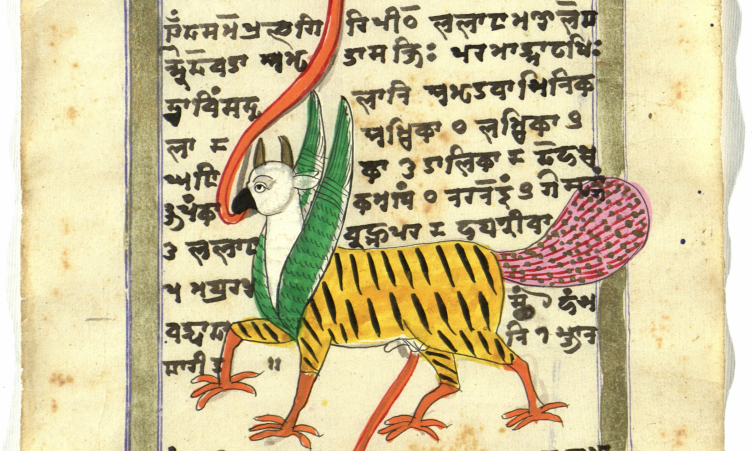
\includegraphics[width=1\textwidth]{pics/Wolpertinger.png}
\caption[The \textit{dehasvarūpa} of \textit{ajapāgāyatrī}]{The \textit{dehasvarūpa} of \textit{ajapāgāyatrī}. The image, reminiscent of a hippogriff, is part of an illustrated Sanskrit manuscript written in the Śāradā script. Preserved as a single large scroll under Acc. No. 1334 at the Oriental Institute in Srinagar (Kashmir), it is entitled \textit{Nāḍīcakra}. The manuscript contains a depiction of the yogic body’s \textit{cakra}s and \textit{nāḍī}s. The text surrounding the figure closely corresponds to the additional material found in manuscript \getsiglum{U2} of the \textit{Tattvayogabindu}. The manuscript reads (diplomatic transcription): \textit{oṃ daśame pūrṇagiripīṭhe lalāṭamaṇḍale candro devatā amṛtāśaktiḥ paramātmā ṛṣiḥ dvāviṃśaddalāni amṛtavāsinikalā 4: ambikā 1 lambikā 2 gha(ṃ)ṭkā 3 tālikā 4 dehasvarūpaṃ kākamukhaṃ 1 naranetraṃ 2 gośṛṅgaṃ 3 lalāṭabrahmapara 4 hayagrīvā 5 mayūramuśchaṃ 6 haṃsacārītani 7 sthāna.}}
	\phantomsection\label{fig_wolpertinger}
      \end{figure}

      \clearpage

  \begin{figure}[ht]
	\centering
  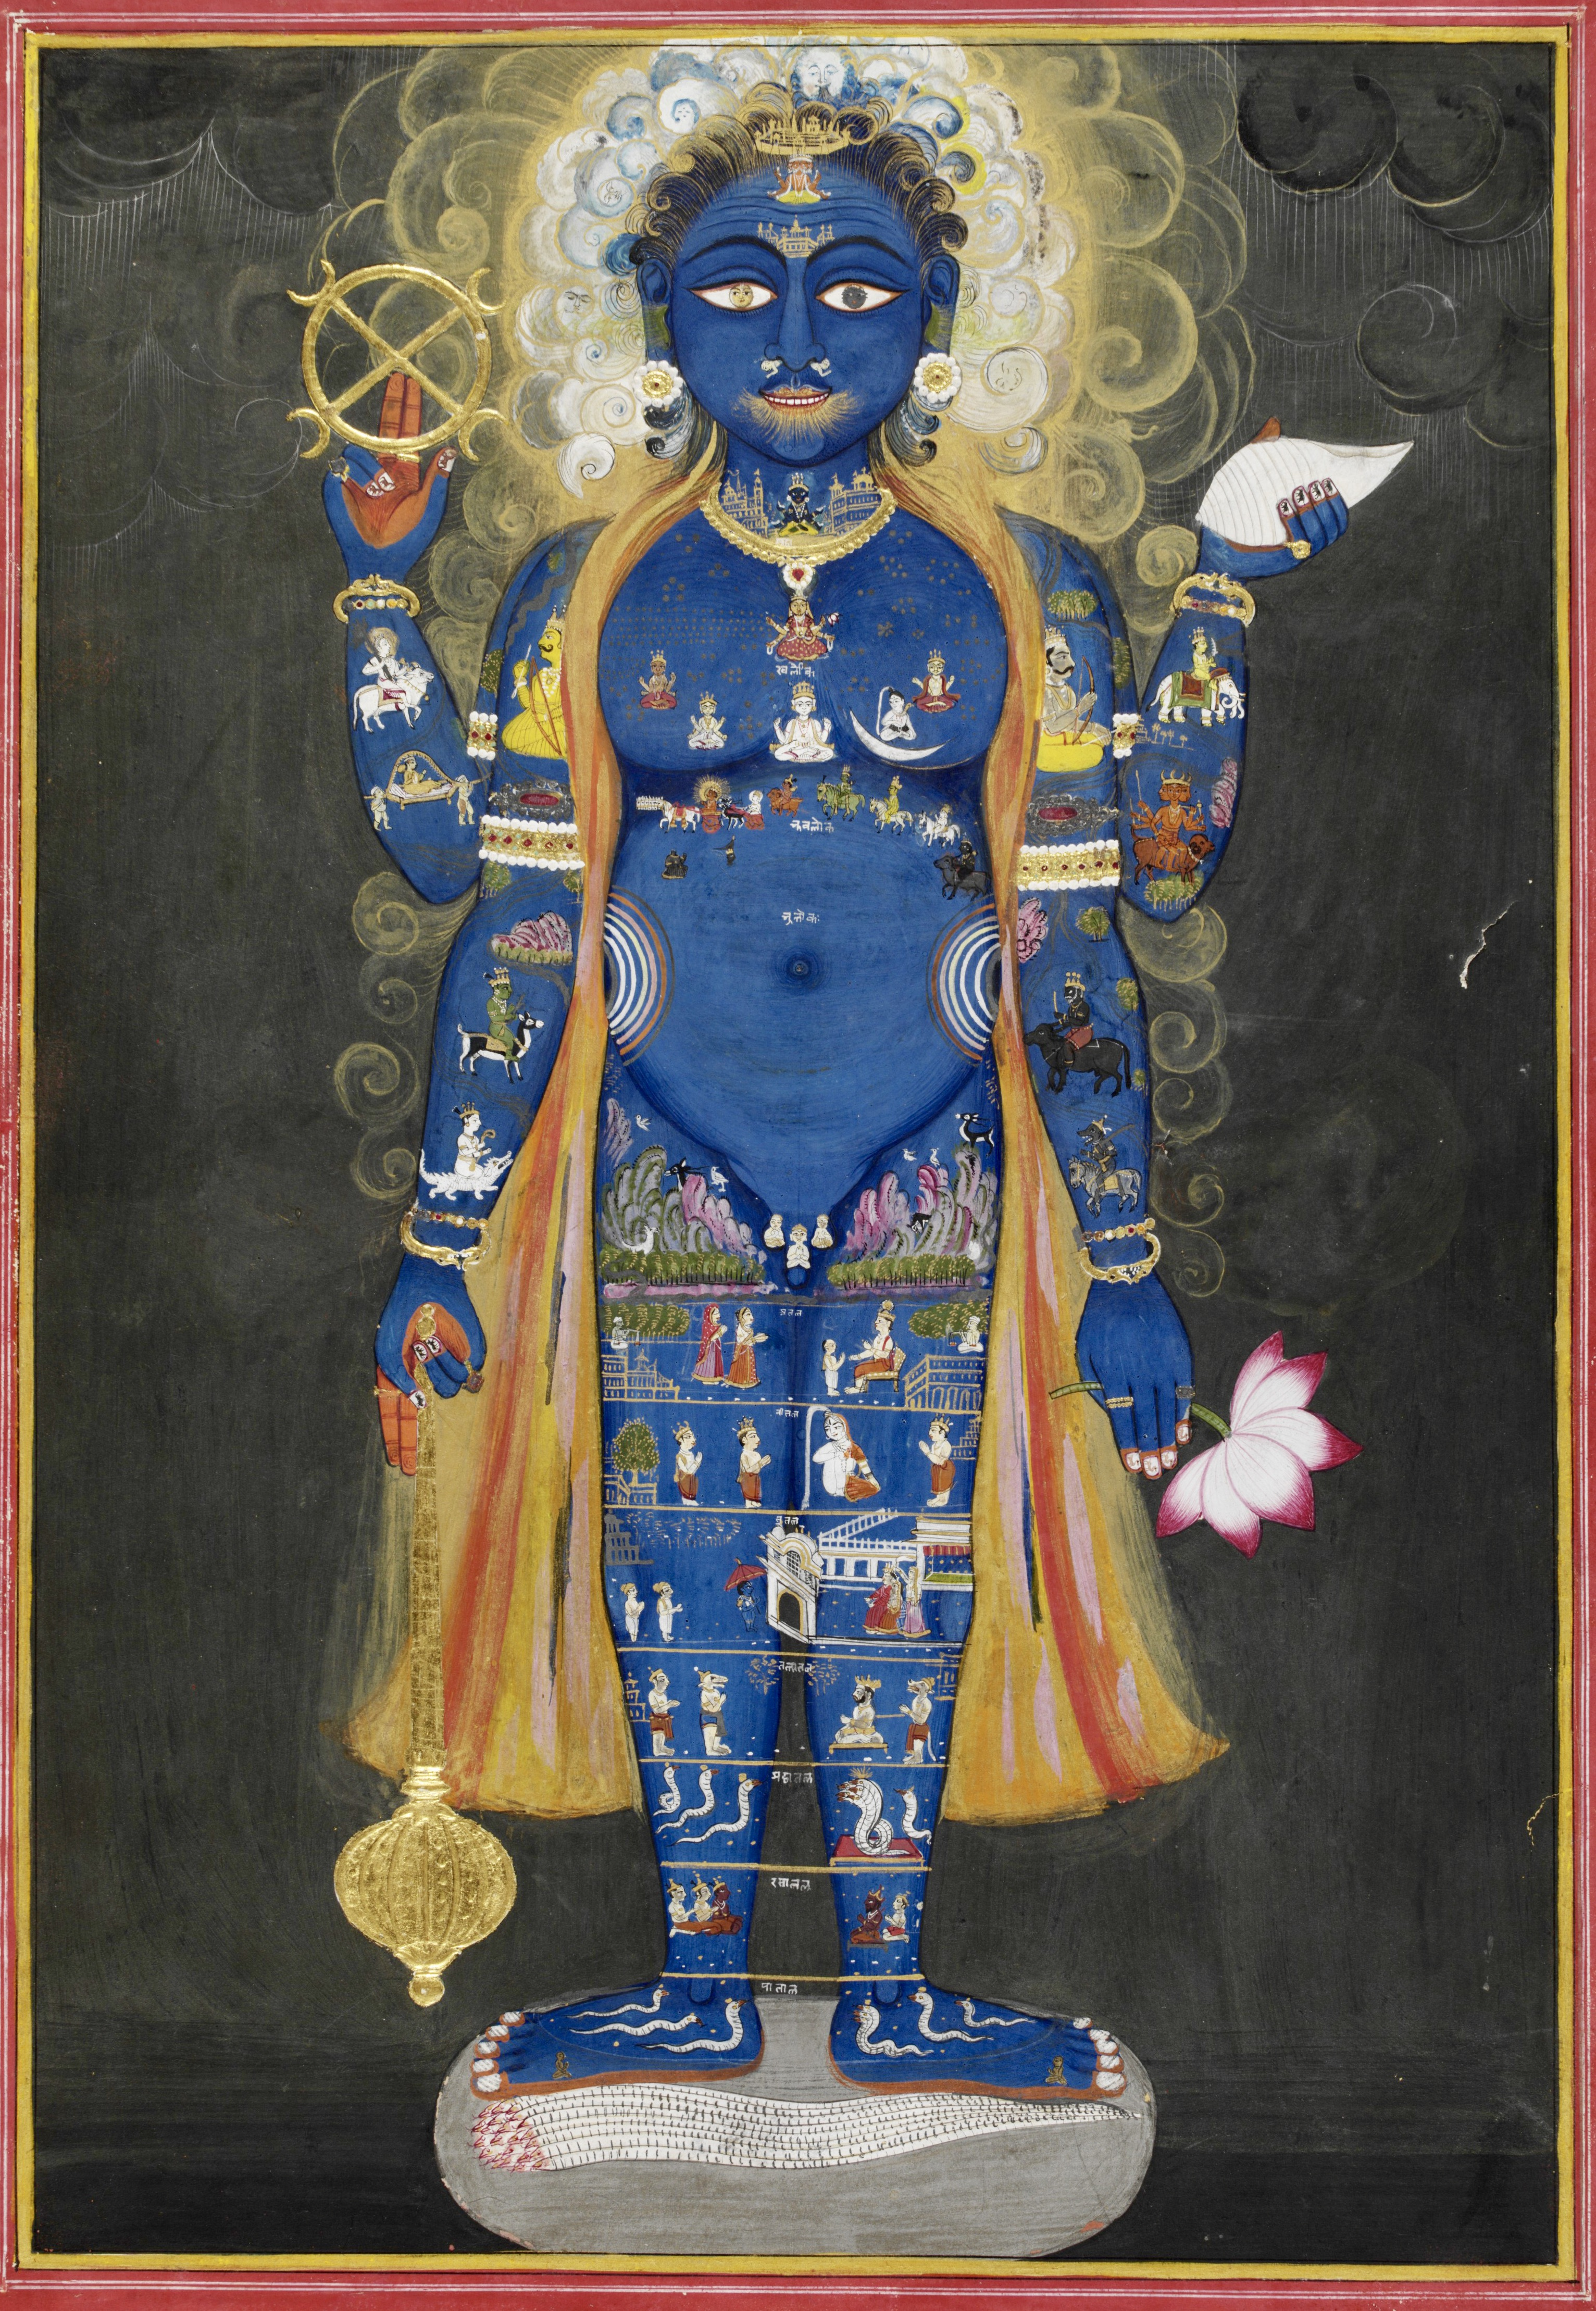
\includegraphics[width=1\textwidth]{pics/Vishnu_Vishvarupa_cropped.jpg}
	\caption{Viṣṇu Viśvarūpa, India, Rajasthan, Jaipur, ca. 1800–1820, Opaque watercolor and gold on paper, 38.5 × 28 cm, Victoria and Albert Museum, London, Given by Mrs. Gerald Clark.}
	\label{fig1}
      \end{figure}
\clearpage
  \begin{figure}[ht]
	\centering
  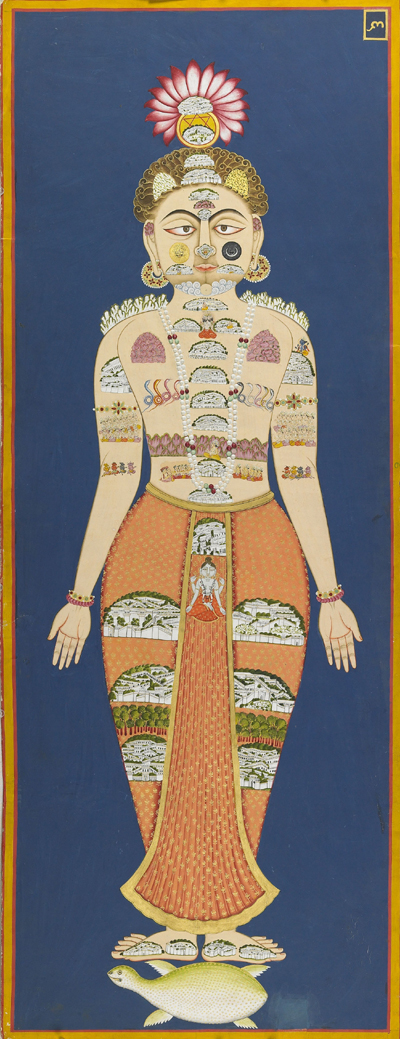
\includegraphics[width=0.5\textwidth]{pics/The_Equivalence_of_Self_and_Universe_(detail),_folio_6_from_the_Siddha_Siddhanta_Paddhati,_(Bulaki),_1824_(Samvat_1881);_122_x_46_cm._Mehrangarh_Museum_Trust..jpg}
	\caption{The Equivalence of Self and Universe (detail), folio 6 from the \textit{Siddhasiddhāntapaddhati} (Bulaki), India, Rajasthan, Jodhpur, 1824 (Samvat 1881), 122 x 46 cm, RJS 2378, Mehragarh Museum Trust.}
	\label{fig2}
      \end{figure}
      % \end{landscape}

      \newpage
      \cleardoublepage
\chapter{Bibliography}
 \label{sec:bibli}
\clearpage
\newpage 
\thispagestyle{empty}
\quad  \addtocounter{page}{-1}

\newrefcontext[sorting=tixel]
\printbibliography[heading=subbibintoc, title=Primary Sources, keyword=primary]

\newrefcontext[sorting=nyt]
\printbibliography[heading=subbibintoc, title=Secondary Literature, keyword=seclit]

\printbibliography[heading=subbibintoc, title=Catalogues, keyword=catalogues]

\printbibliography[heading=subbibintoc, title=Online Sources, keyword=onlinesource]

\end{document}


%%% Local Variables:
%%% mode: latex
%%% TeX-master: t
%%% End:
